\documentclass{sigchi}

% Use this command to override the default ACM copyright statement
% (e.g. for preprints).  Consult the conference website for the
% camera-ready copyright statement.

%% EXAMPLE BEGIN -- HOW TO OVERRIDE THE DEFAULT COPYRIGHT STRIP -- (July 22, 2013 - Paul Baumann)
% \toappear{Permission to make digital or hard copies of all or part of this work for personal or classroom use is      granted without fee provided that copies are not made or distributed for profit or commercial advantage and that copies bear this notice and the full citation on the first page. Copyrights for components of this work owned by others than ACM must be honored. Abstracting with credit is permitted. To copy otherwise, or republish, to post on servers or to redistribute to lists, requires prior specific permission and/or a fee. Request permissions from permissions@acm.org. \\
% {\emph{CHI'14}}, April 26--May 1, 2014, Toronto, Canada. \\
% Copyright \copyright~2014 ACM ISBN/14/04...\$15.00. \\
% DOI string from ACM form confirmation}
%% EXAMPLE END -- HOW TO OVERRIDE THE DEFAULT COPYRIGHT STRIP -- (July 22, 2013 - Paul Baumann)

% Arabic page numbers for submission.  Remove this line to eliminate
% page numbers for the camera ready copy
% \pagenumbering{arabic}

% Load basic packages
\usepackage{balance}  % to better equalize the last page
\usepackage{graphics} % for EPS, load graphicx instead 
\usepackage[T1]{fontenc}
\usepackage{txfonts}
\usepackage{mathptmx}
\usepackage[pdftex]{hyperref}
\usepackage{color}
\usepackage{booktabs}
\usepackage[utf8]{inputenc}
\usepackage{textcomp}
% Some optional stuff you might like/need.
\usepackage{microtype} % Improved Tracking and Kerning
% \usepackage[all]{hypcap}  % Fixes bug in hyperref caption linking
\usepackage{ccicons}  % Cite your images correctly!
% \usepackage[utf8]{inputenc} % for a UTF8 editor only

% If you want to use todo notes, marginpars etc. during creation of your draft document, you
% have to enable the "chi_draft" option for the document class. To do this, change the very first
% line to: "\documentclass[chi_draft]{sigchi}". You can then place todo notes by using the "\todo{...}"
% command. Make sure to disable the draft option again before submitting your final document.
\usepackage{todonotes}

% Paper metadata (use plain text, for PDF inclusion and later
% re-using, if desired).  Use \emtpyauthor when submitting for review
% so you remain anonymous.
\def\plaintitle{SIGCHI Conference Proceedings Format}
\def\plainauthor{First Author, Second Author, Third Author,
  Fourth Author, Fifth Author, Sixth Author}
\def\emptyauthor{}
\def\plainkeywords{Authors' choice; of terms; separated; by
  semicolons; include commas, within terms only; required.}
\def\plaingeneralterms{Documentation, Standardization}

% llt: Define a global style for URLs, rather that the default one
\makeatletter
\def\url@leostyle{%
  \@ifundefined{selectfont}{
    \def\UrlFont{\sf}
  }{
    \def\UrlFont{\small\bf\ttfamily}
  }}
\makeatother
\urlstyle{leo}

% To make various LaTeX processors do the right thing with page size.
\def\pprw{8.5in}
\def\pprh{11in}
\special{papersize=\pprw,\pprh}
\setlength{\paperwidth}{\pprw}
\setlength{\paperheight}{\pprh}
\setlength{\pdfpagewidth}{\pprw}
\setlength{\pdfpageheight}{\pprh}

% Make sure hyperref comes last of your loaded packages, to give it a
% fighting chance of not being over-written, since its job is to
% redefine many LaTeX commands.
\definecolor{linkColor}{RGB}{6,125,233}
\hypersetup{%
  pdftitle={\plaintitle},
% Use \plainauthor for final version.
%  pdfauthor={\plainauthor},
  pdfauthor={\emptyauthor},
  pdfkeywords={\plainkeywords},
  bookmarksnumbered,
  pdfstartview={FitH},
  colorlinks,
  citecolor=black,
  filecolor=black,
  linkcolor=black,
  urlcolor=linkColor,
  breaklinks=true,
}

% create a shortcut to typeset table headings
% \newcommand\tabhead[1]{\small\textbf{#1}}

% End of preamble. Here it comes the document.
\begin{document}

\title{\plaintitle}

\numberofauthors{4}
\author{
  \alignauthor{Thomas Nyegaard-Signori\\
    \email{sfq340@alumni.ku.dk}}\\
  \alignauthor{Tobias Carlos Tvarnø\\
    \email{e-mail address}}\\
  \alignauthor{Tor-Salve Dalsgaard\\
    \email{e-mail address}}\\
  \alignauthor{Enes Golic\\
    \email{e-mail address}}\\
}

\maketitle

\begin{abstract}
Every submission should begin with an abstract of about 150 words,
followed by a set of Author Keywords and ACM Classification
Keywords. The abstract and keywords should be placed in the left
column of the first page under the left half of the title. The
abstract should be a concise statement of the problem, approach, and
conclusions of the work described. It should clearly state the paper's
contribution to the field of HCI\@.
\end{abstract}

\category{H.5.m.}{Information Interfaces and Presentation
  (e.g. HCI)}{Miscellaneous} \category{See
  \url{http://acm.org/about/class/1998/} for the full list of ACM
  classifiers. This section is required.}{}{}

\keywords{\plainkeywords}

% !TeX root = ../project.tex

\section{Introduction}
This report focuses on an application for the newly released Microsoft Hololens. The Hololens was released around march 2017, and the fact that the product is in its infant stage and is based on a very new technology opens up possibilities and removes any preconceived notions about which applications and uses the Hololens might have.\\
The technology is relevant with regards to mobile computing in one very apparent way, in that it is a wearable, computing unit. Other than that, it offers alternate reality (AR) possibilities because of its partly see-through screens and user tracking. Since the Hololens is still a new technology, the mobility and computing power of the product will most likely increase, making it resemble a ubiquitous computer more and more. This evolution of mobile computing was one of the reasons that the Hololens was chosen to develop on in the first place.\\\\
The application this report will cover revolves around LEGO. LEGO is a way for kids and adults to build constructions, vehicles and scenery, all in a very physical and three-dimensional way. This, then, seemed like a natural choice for an AR application, since the application layer between the user and the world could expand naturally on the possibilities and limitations of the physical, "real-world" LEGO.\\
The application in itself should be a sort of digital playground in which a user could interact with LEGO in ways they would find natural. Sticking pieces together the way they do in real life, stacking and constructing, all interactions that the user knows well from having played around with real LEGO. This was done using interaction through a virtual tablet, known as the "Generator board" and simple drag-and-drop with the bricks. We end up with a rough prototype which helped us discover the pitfalls and consideration concerning a LEGO implementation in an AR enviroment. 

\section{Sketching}
The structure can look like this:
\begin{itemize}
	\item Present the chosen design challenges and some of the initial concerns in the beginning phase
	\item Each challenge is outlined with:
		\begin{itemize}
			\item Sketches
			\item Design thoughts for the sketch - what was the thought behind this sketch?
			\item summary of the group discussion for this case - what worked, what didn't and why?
		\end{itemize}
	\item Conclude what the final sketches are - what do they accomplish, and what do they lack(maybe reference what might be discussed in future work)?
\end{itemize}
\subsection{How do we access the application? (Menu)}
The menu is an essential part of any application. It outlines the possibilities for the user in a simple fashion. The menu is something every user has experience with, as it is the first thing a user is met with when running an application. This means that the menu has to contain of certain classic elements.\par A user needs a way to close the application. On mobile phones nowadays this can be done with 'return' buttons on the phone, but all applications generally have a built in exit function.\par
The user also needs to have some sort of options menu, and guidelines. This is a must for this application. Stacking LEGO seems simple and intuitive, but all the operations and possibilities is something that can confuse a potential user. \par
Lastly the menu needs to have an easy access to the LEGO session itself. It shouldn't be complicated for the user to start a new LEGO session, meaning that this action should be as intuitive as it gets.\par
\begin{center}
	Insert sketch 1:
\end{center}

\subsection{The main menu screen}
The initial ideas for the main menu were generated following the 'x plus x' sketch generation principle outlined in the course. In the case of the sketching done for the main menu, a '5 plus 5' scheme was used. One common theme in the sketching of the main menu was separation of the design of the menu and the interaction with the menu, and the difficulties with making that separation. In quite a few of the earlier sketches, what was being sketched was more a way of interacting with the menu rather than the design of the menu itself.\\
\\
It became apparent that the menu had to use the gestures given from Hololens, ie., the bloom gesture. Since a fixed main menu screen could lead to different problems, such as blocking precious field of view, and a menu screen fixed to the world could be forgotten and overlooked, a gesture-activated main menu was the prefered interaction.

\subsection{The generator board}
After discussing menus in the context of the Hololens, it became apparent that there was a need for a menu that could be placed and interacted with in the real world. Using the tracking capabilities of the Hololens, different designs of the so called 'generator board' came up. The main purpose of the generator board is to generate blocks that the user can then drag out of the predefined spawning space.\\
\\
The idea came up that a menu with the same look and functionality of a tablet device could make interaction natural for the user. Having the ability to pick up, move and place the menu on a surface like a table or the floor seemed like a natural way of approaching the problem. The idea can be seen in a very early sketch in figure (HVILKEN FIGUR?):\\


\begin{figure}
\centering
  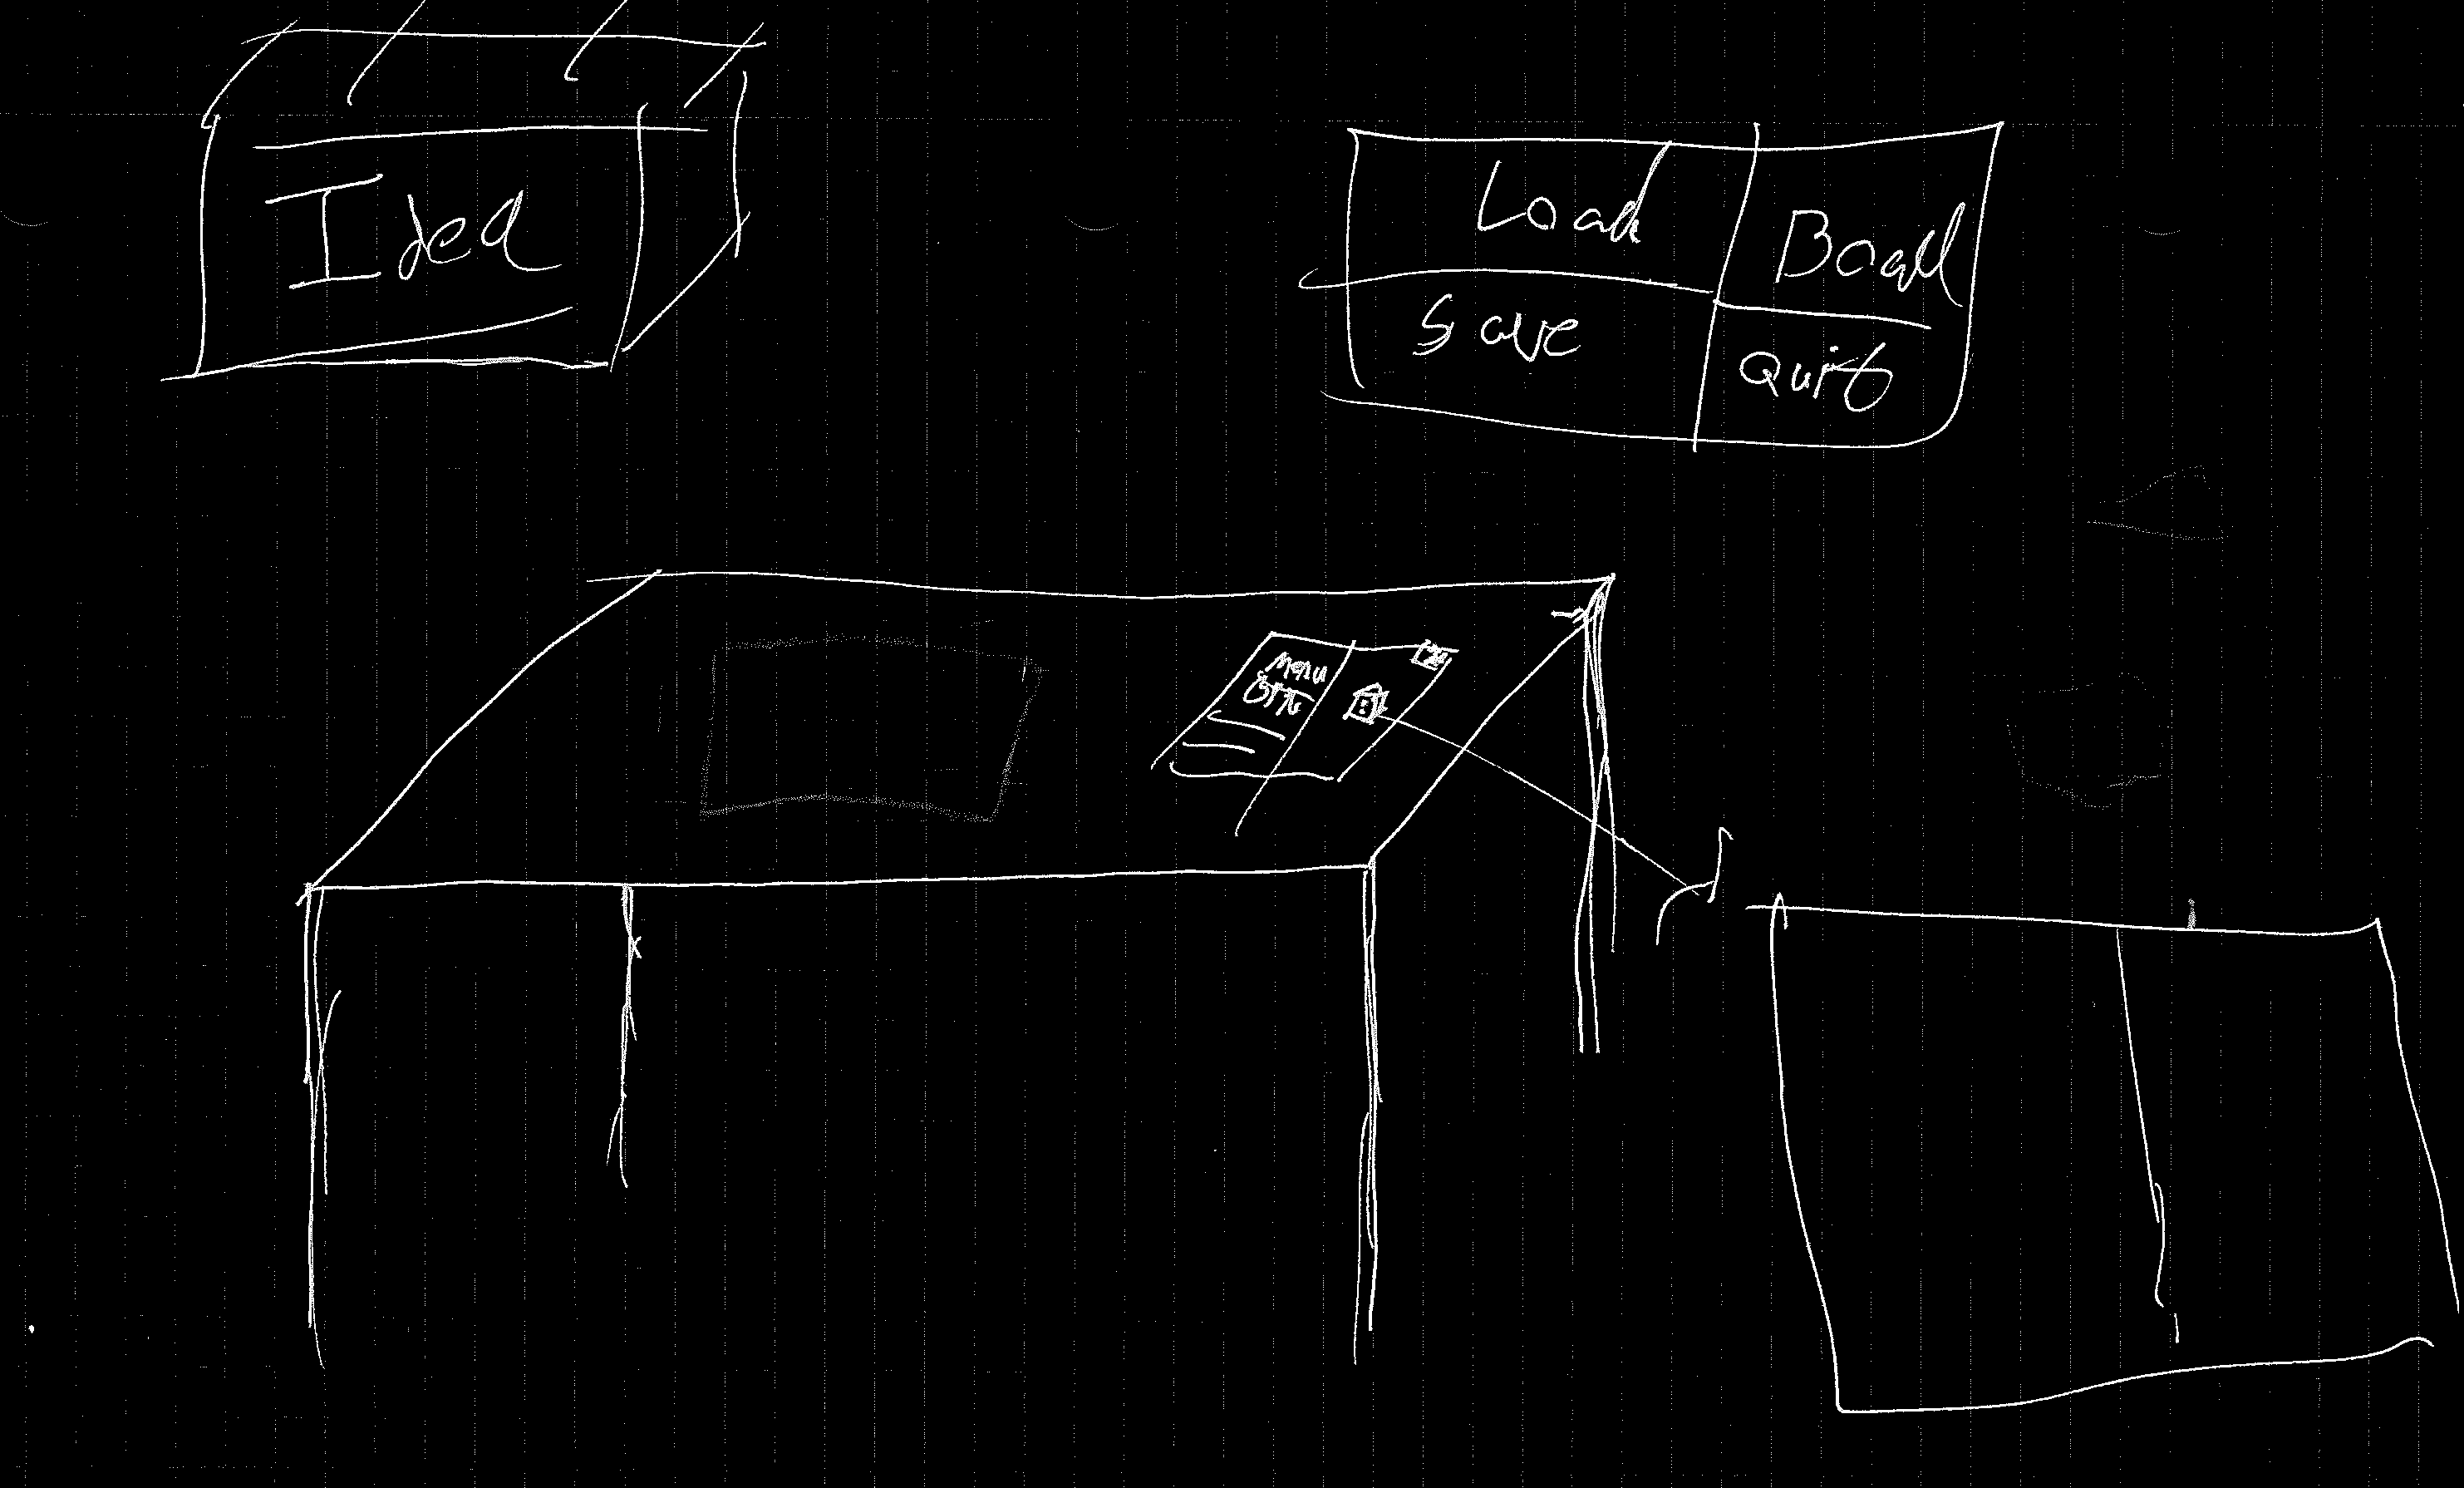
\includegraphics[width=0.9\columnwidth]{figures/Generator/gen6.png}
  \caption{Skriv lidt lækert her. }~\label{fig:genboard}
\end{figure}


% !TeX root = ../proceedings.tex

\section{Design Challenges}
\subsection{Accessibility}
To manoeuvre around in any application, a menu is needed. The menu is something every user has experience with and it is the first thing a user is met with when running an application. This means that the menu has to consist of certain classic elements.\par A user needs a way to close the application. On mobile phones nowadays this can be done with 'return' buttons on the phone, but applications generally have a built in exit function.\par
The user also needs to have some sort of options menu and guidelines. Stacking LEGO seems simple and intuitive, but all the operations and possibilities is something that can confuse a potential user. \par
Lastly it shouldn't be complicated for the user to start a new LEGO session. \par
\subsection{A Main Menu}
To achieve accessibility a '5 plus 5' sketch generation session was held. Initially we thought about this application as a game, therefore the user would typically be met by a main menu screen, just as figure \ref{fig:menu8} illustrates.
\begin{figure}[h]
	\centering
	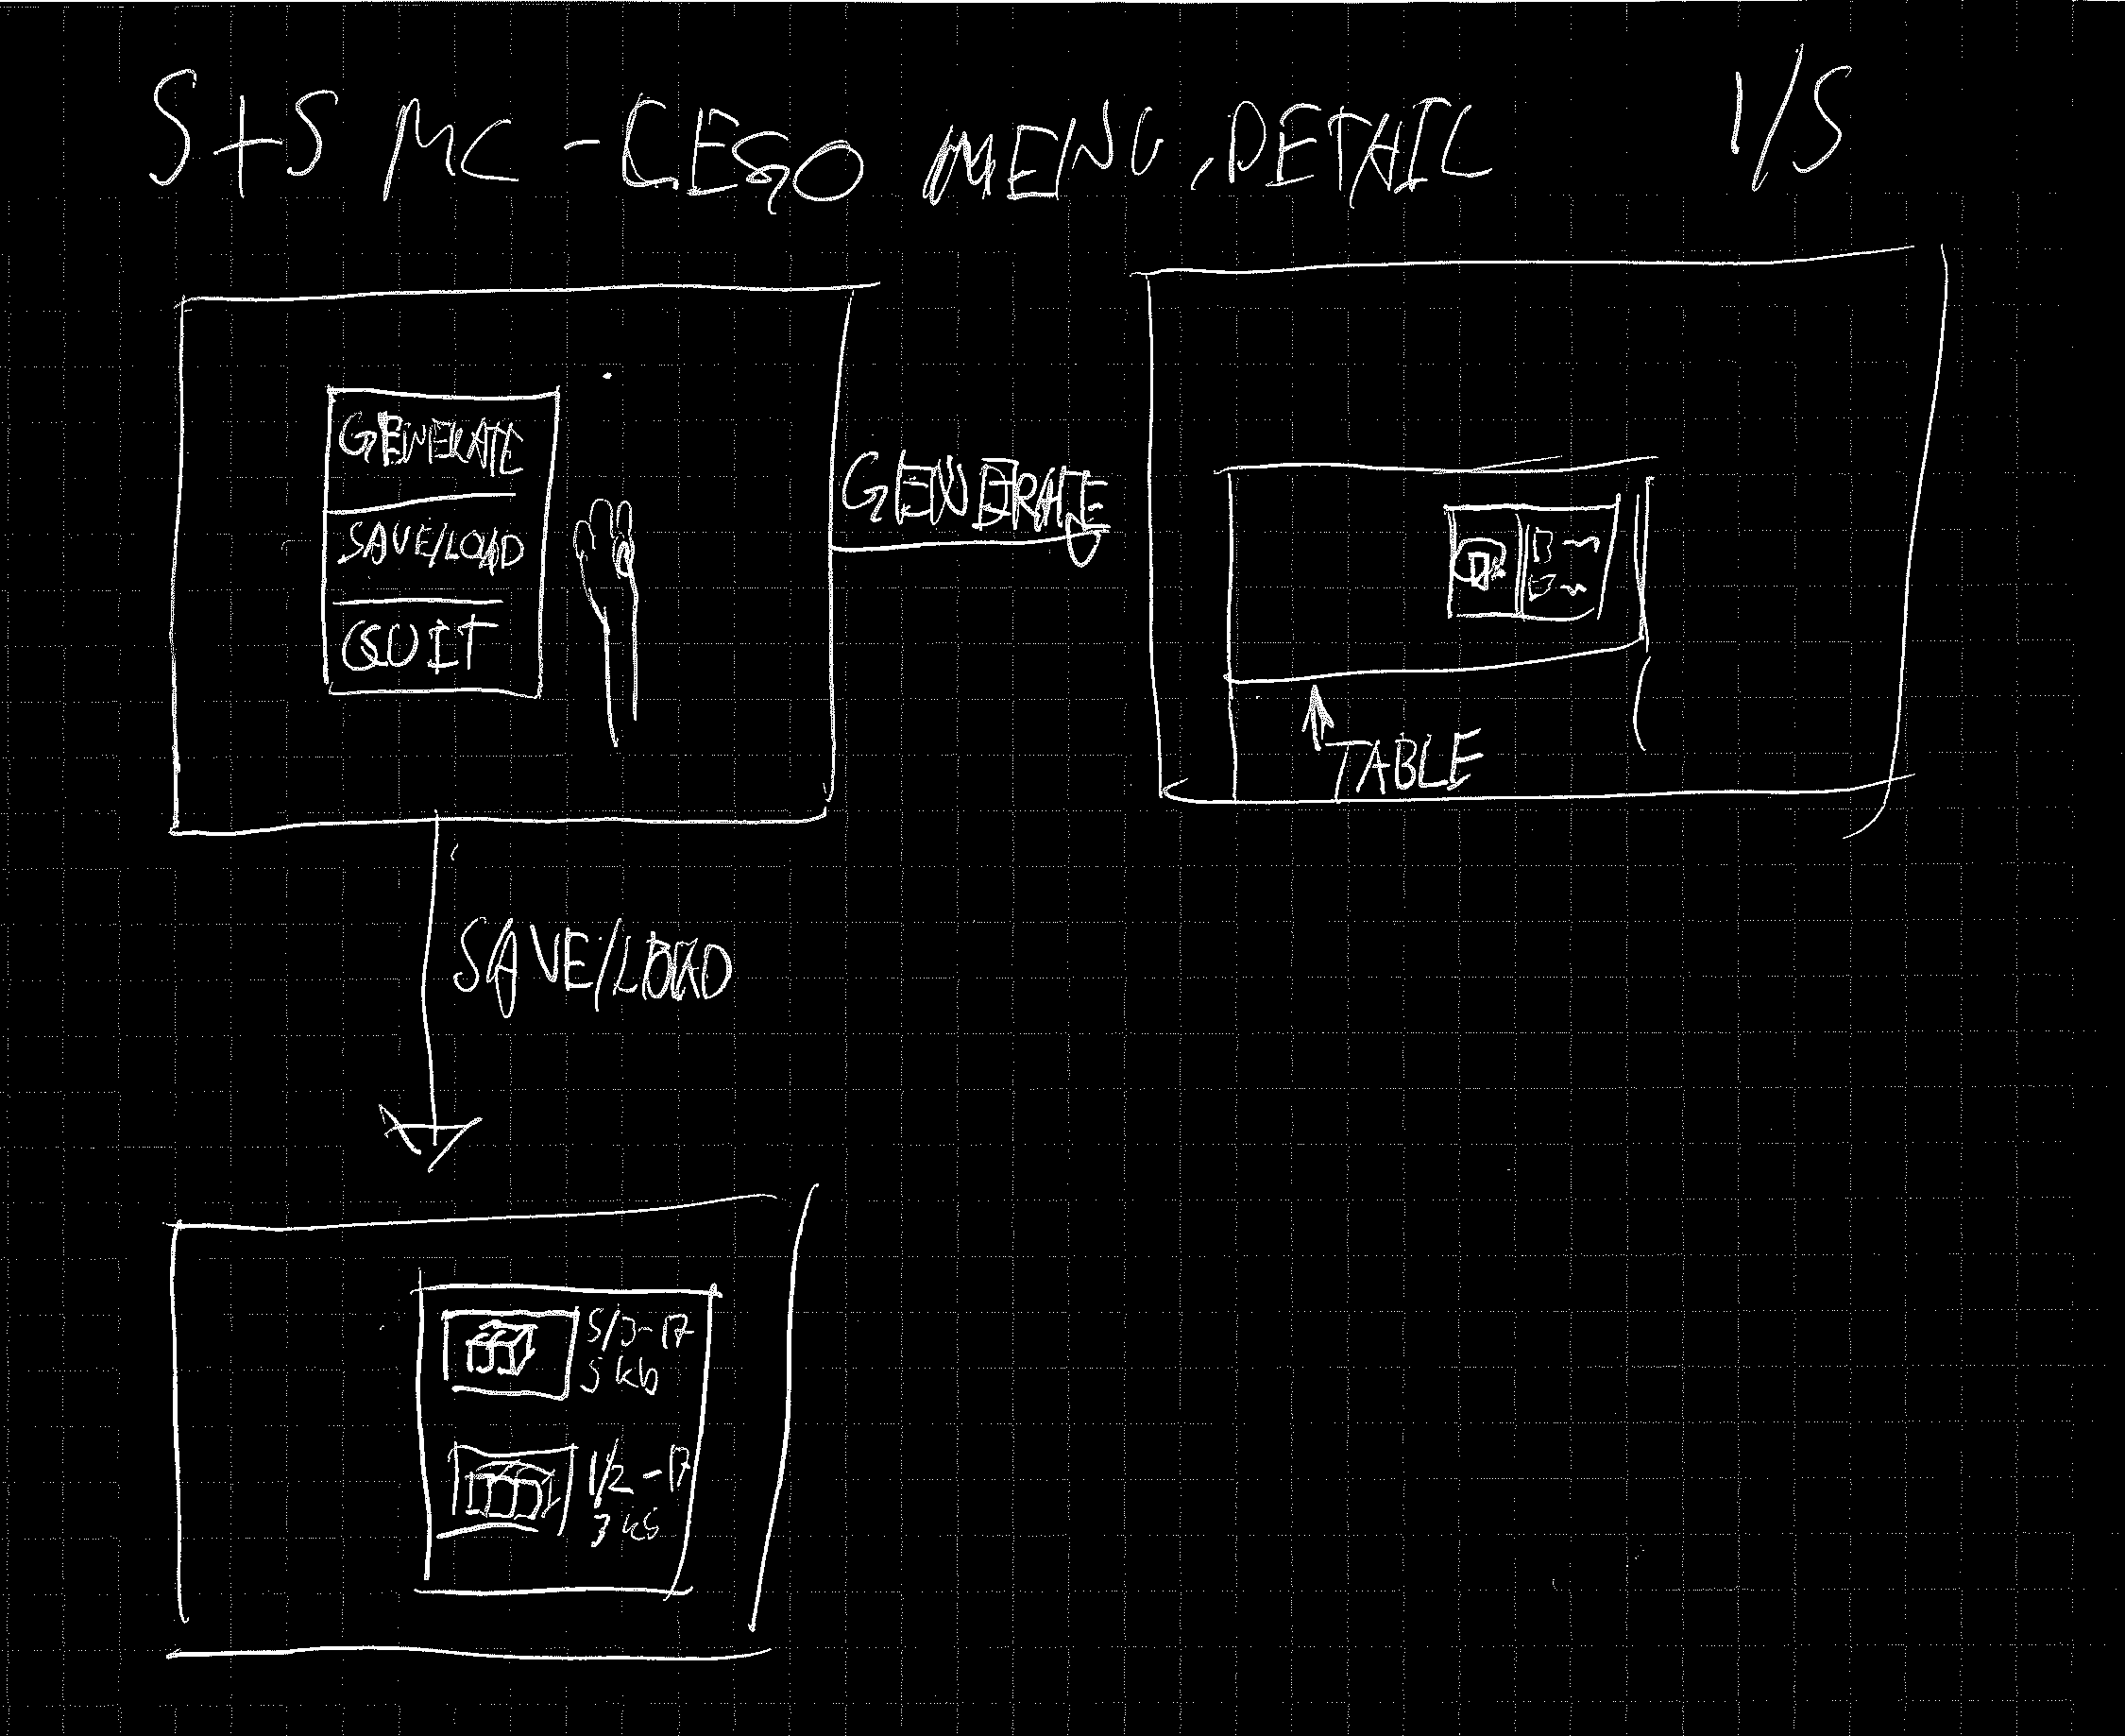
\includegraphics[width=0.7\linewidth]{figures/Menu/menu8}
	\caption{The first idea of a seperate Main Menu screen}
	\label{fig:menu8}
\end{figure}
The user would open the Hololens application, and be met with a menu screen, where actions such as generating a play area, loading and saving a game and a way to quit the application were possible. \par
One common theme in the sketching of the main menu was separating the design of the menu and the interaction techniques with the menu. This led to some sketches being focused on the interaction, such as figure \ref{fig:menugesture} depicts, and other sketches that solely focused on the menu design.\par
\begin{figure}[h]
	\centering
	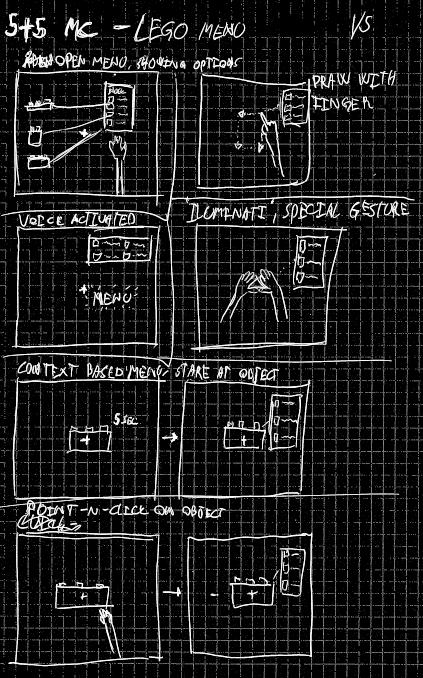
\includegraphics[width=0.7\linewidth]{figures/Menu/menu5}
	\caption{A focus on gestures rather than design, impacted the design. The figure shows 5 different ways of creating an interactive menu for the user to use.}
	\label{fig:menugesture}
\end{figure}
\par
The possibilities with the HoloLens gestures and the augmented reality made it apparent that the menu had to be movable, either by closing and opening with the gestures available, or being able to move it around the play area. 
\subsection{The Generator Board}
After discussing menus in the context of the Hololens, it became apparent that there was a need for a menu that could be placed and interacted within the real world. This menu should only interact inside the play area, and have functions tied to the bricks. Figure \ref{fig:genboard1} is a sketch of what functionalities the generator board could have.
\begin{figure}[h]
	\centering
	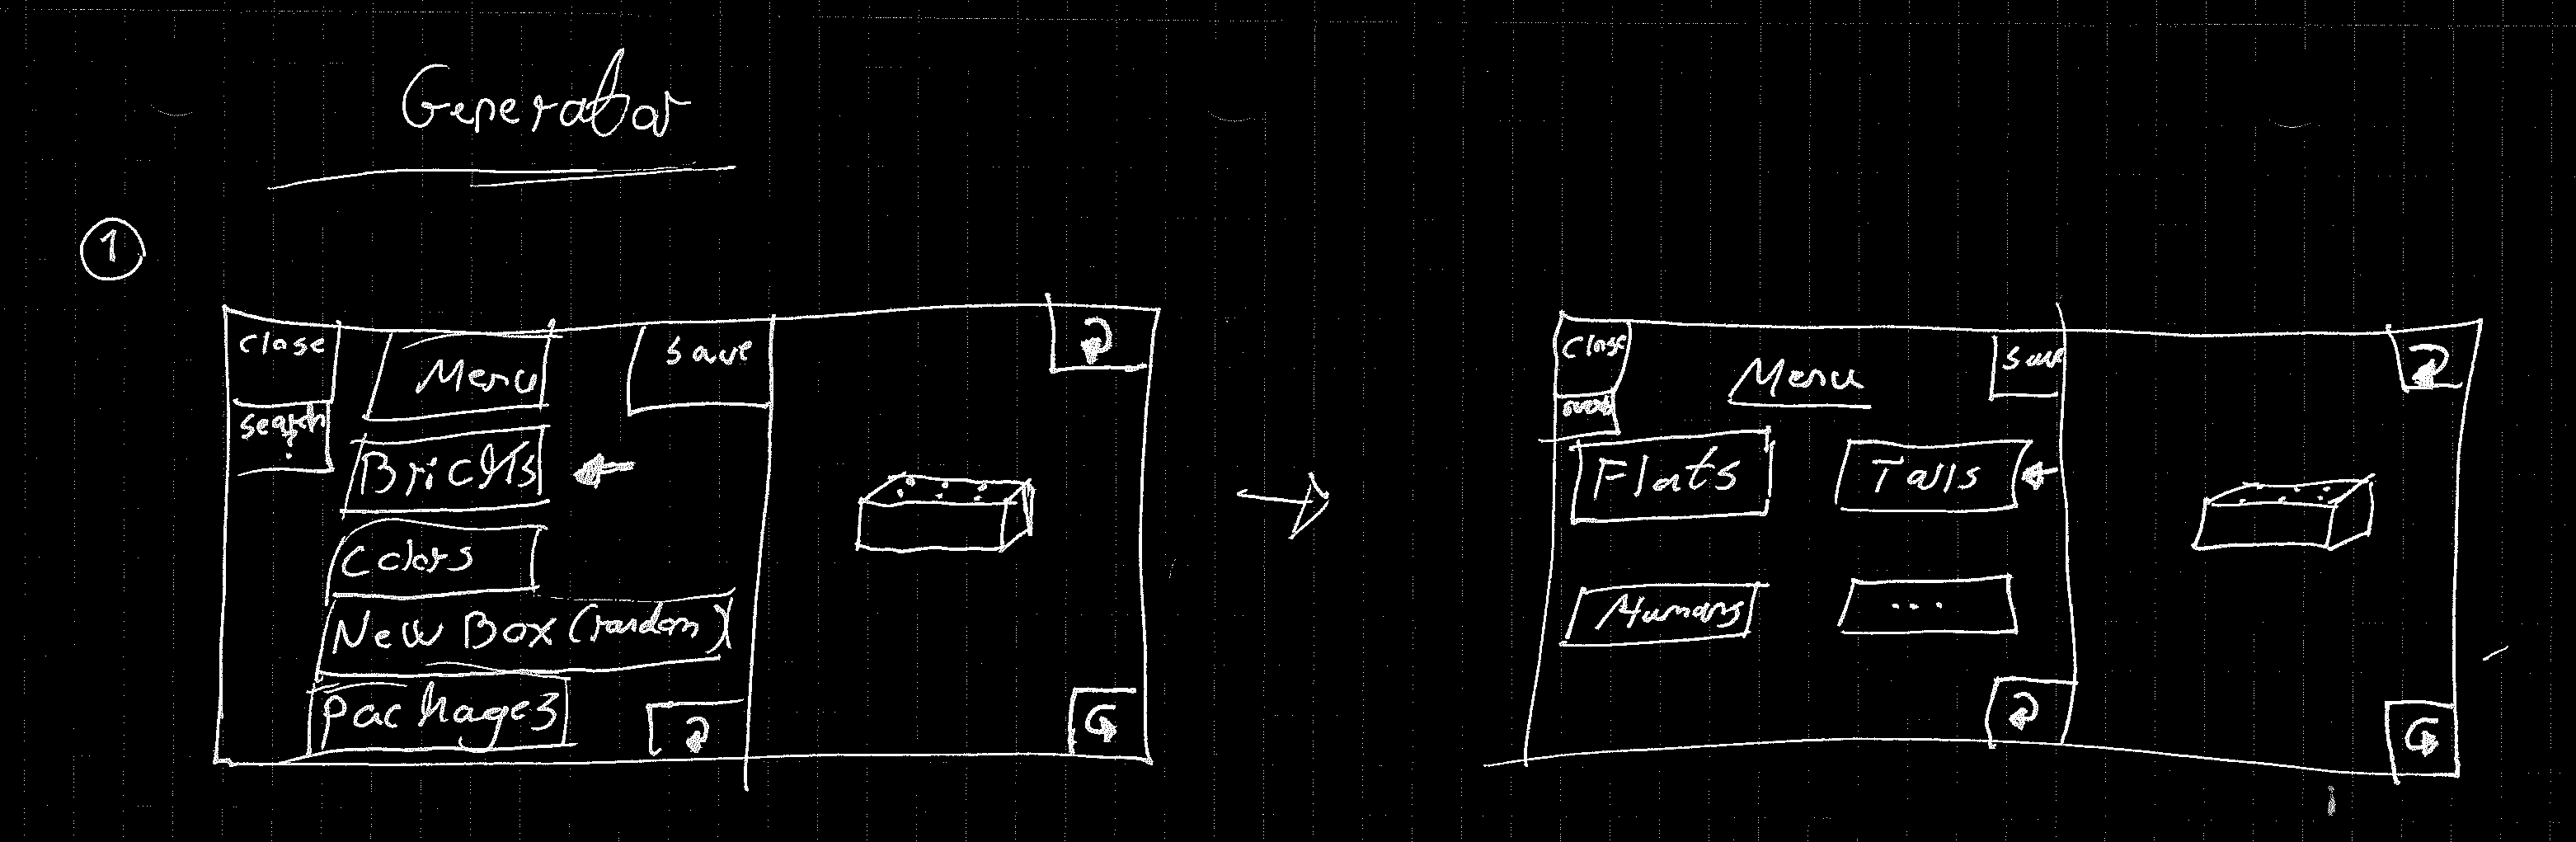
\includegraphics[width=0.7\columnwidth]{figures/Generator/gen5.png}
	\caption{An initial sketch of how the generator board could look like. The menu screen has alot of functionalities, and the actions chosen happen on the right side.}~\label{fig:genboard1}
\end{figure}
The generator board should be have functionalites that can alter the blocks, but also needs to be interactive and moveable in the play area.\par
Figure \ref{fig:gentablet} illustrates how the generator board is placed on a table and used for generating bricks.
\begin{figure}[h]
	\centering
	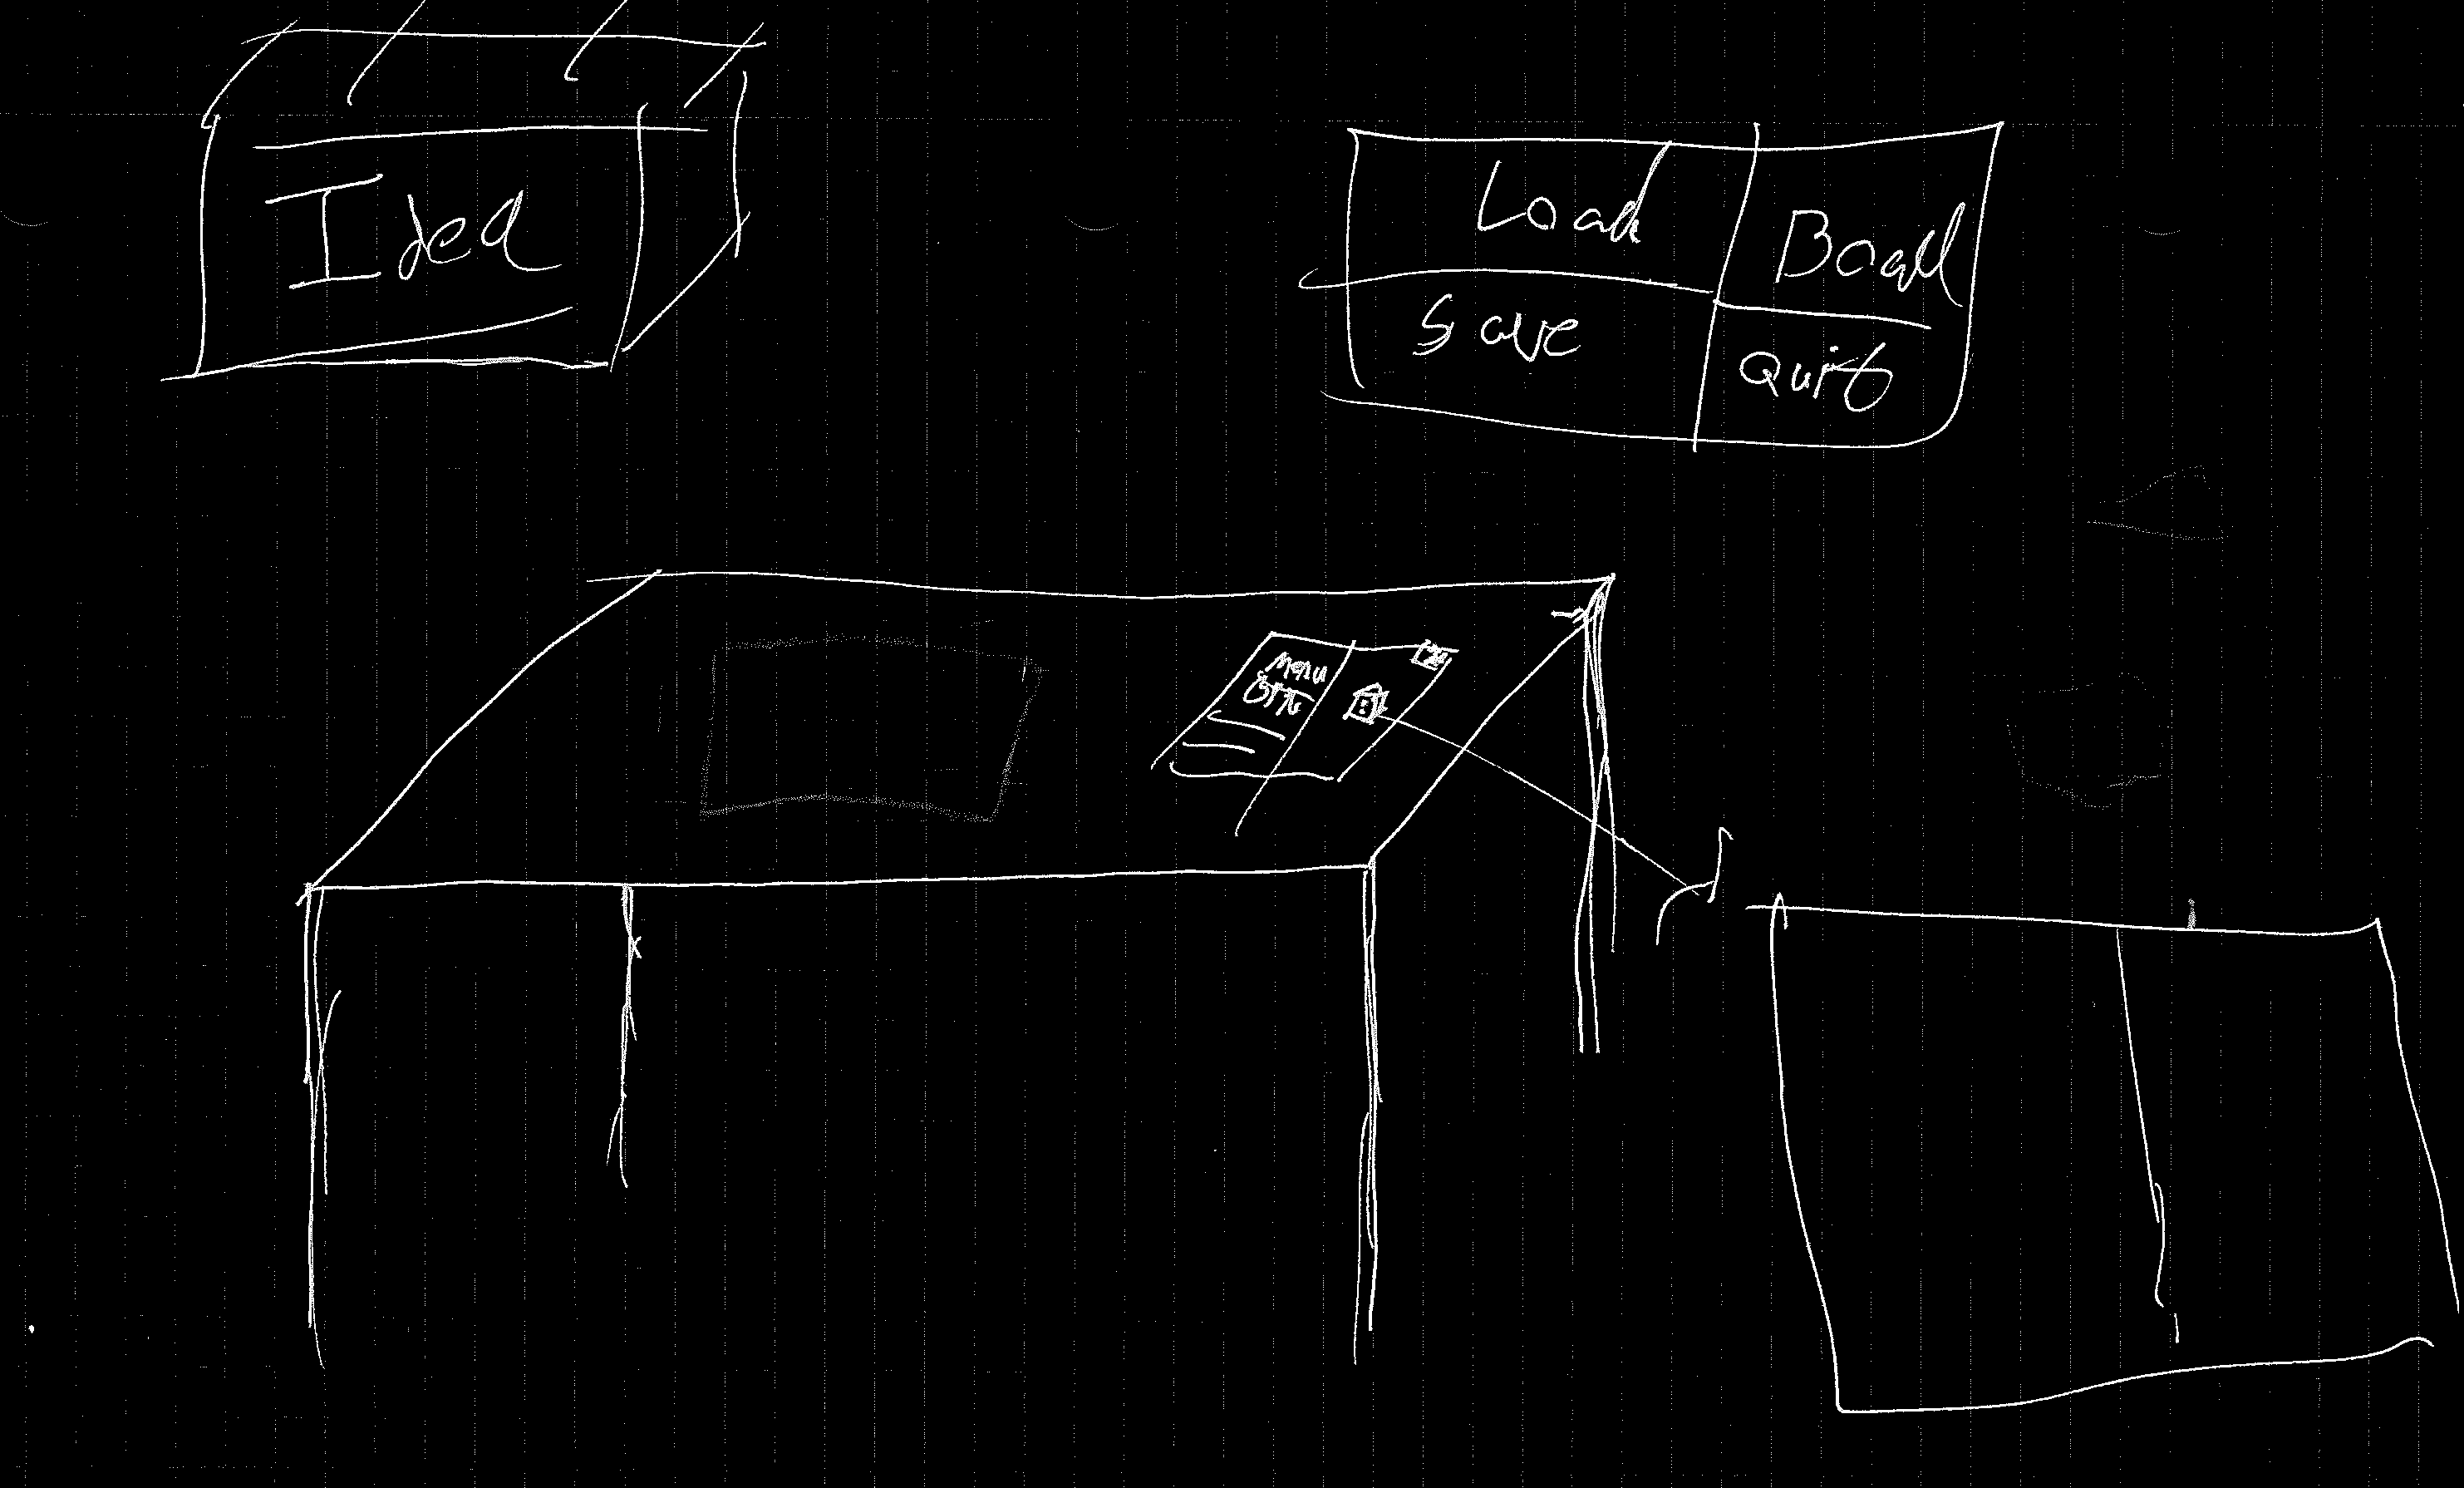
\includegraphics[width=0.7\columnwidth]{figures/Generator/gen6.png}
	\caption{First sketch of the generator board as a movable object. Here placed on the table, spawning blocks on the table.}~\label{fig:gentablet}
\end{figure}
We designed the generator board as a tablet device. Being a solid familar object, makes it more intuitive and natural for the user to interact with. To lift, move and place the tablet on a surface is a simple and familiar task for the user. To accompany the tablet device, a simple interface was designed. The interface only needed simple function all tied to spawning lego bricks. The user can spawn bricks of different types, change colors and saving/loading a play scene.
\subsection{Design Decisions}
\begin{figure}[h]
	\centering
	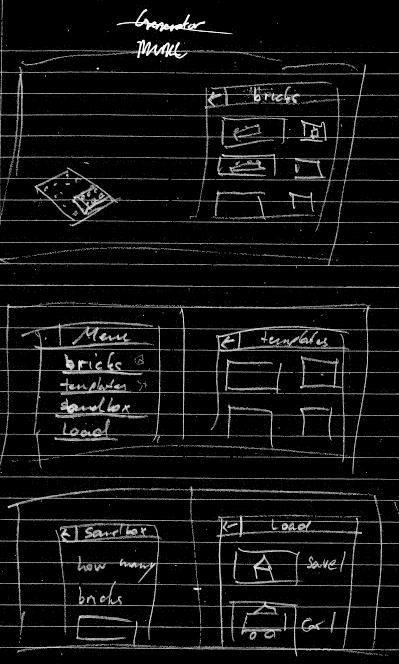
\includegraphics[width=0.5\columnwidth]{figures/Menu/menu1.png}
	\caption{Initial Main Menu screen with big buttons, simple interaction and short descriptions.}~\label{fig:genboard}
\end{figure}
During the sketching phase, several design choices were discussed. One of the very first concerns was the overall look of the main menu. The choice of big buttons, clear visual cues and short textual descriptions was present in almost all of the sketches in the early design phase, as seen in figure \ref{fig:genboard}. The generator board needed to have the same simple design. We decided The menus should not be overcomplicated, but not sparse in functions either.\par
As the development of the application progressed it became more  apparent that an actual main menu was not necessary. All the interactions needed for the prototype could be implemented  the tablet looking generator board and could ease user interaction with the application. Instead of going through a main menu and then having the generator which contains the functionality for working with the LEGO bricks, spawning the generator board at the application start up and "cutting out the middleman" seemed as a natural choice for this prototype. Granted, with an eventual increase in functionality and complexity of the application, a root/main menu might prove useful as to not clutter the users experience when they are building as opposed to when they are in the main menu setting options, loading scenarios, downloading templates etc. 



% !TeX root = ../project.tex

\section{Holotoolkit}
The main package (?) used for developing for the Hololens in this project was the HoloToolkit-Unity. This package comes with some premade functionality to ease the interaction with the Hololens and is an open source toolkit made by Microsoft to speed up any development for their new platform (quote dem måske?).\\
\\
The toolkit contains seven feature areas, of those spatial mapping and input were of most interest to us. We used the spatial mapping part of the toolkit to be able to "digitize" the world and make our application able to track surfaces so as to place our generator board on real world surfacs instead of having it float in mid air. This connection between the real-world and digital playground created in our application was essential, both to the experience but also to be able to call our application alternate reality. (SKRIV MERE TEKNISK NÅR VI VED HVAD FUCK DER FOREGÅR).\\
\\
The input part of the toolkit allows us to track the gaze and the users interaction with the objects in the application, be it buttons, bricks or the generator board. This tracking is done by shooting a ray from the users gaze (the middle of the screen on the Hololens in our case) and checking whether any colliders, object hitboxes, were hit. This raycasting, as its called, is intuitive since it uses the line of sight from the user to any object in the gameworld, so whatever you can see, you can interact with.\\
More specifically, the orientation and position of the Hololens with regards to the objects in the gameworld is maintained by a GazeManager from the HoloToolkit and the cursor is then placed on the vector originating from the users gaze by a CursorManager. 

% !TeX root = ../proceedings.tex

\section{Future work}

\subsection{Hypothesis specific}
To work with these hypotheses, more tests would have to be conducted, but also the application stability would have to improve dramatically. Users have to feel confident in the application so as to reveal any problems with AR interaction methods as a whole, so that any frustrations and considerations are directed against AR instead of AR AND the application.\\
\\
With regards to H2, tests showed that brick size, ease of access through the menu and a general handholding of the user (in our case, bricks being locked in rotation and snapping to a virtual grid) improved the LEGO experience in an AR setting. Since the technology is not fully developed it is difficult to specify best parameters such as brick size and functionalities that would improve precision. The test subjects showed a general consensus in that LEGO was suitable for AR. One problem is that they only had one point of reference, our high fidelity, but unfinished prototype, and thus it becomes a very subjective matter whether the brick size is actually of an appropriate size or if LEGO as a whole makes sense in AR.\\
One way of narrowing down specific parameters would be a comparative approach to testing, ie. a prototype with different bricks sizes, functionalities and input methods. 

\subsection{Application specific}
To combat the issue with the size of actual LEGO and the complexity available in this scale a virtual magnifying glass could be envisioned. Using a special gesture, a certain area of the LEGO bricks could be brought into view using a secondary "screen", a menu that could show a zoomed in version of the actual view the user has, such as a magnifying glass.\\
\\
The number of input methods implemented into the HoloLens is limited and this is what a test subject criticized. Thus an extension of the input methods is an obvious next step to take. Here the choice of extensions ranges from implementing more hand gestures to using methods such as WatchSense \cite{watchsense}, which utilizes SmartWatches and gestures on the back of the hand to provide a new interaction method. \\
\\
There is a severe shortage of bricks available in the prototype. Anyone who considers an AR LEGO application will soon have to think of which set of blocks or types they would include. The amount of distinctive LEGO bricks is staggeringly high, and this sort of work would probably benefit greatly from working together with LEGO as to get dimensions and oddities right. This work would also make such an application much more attractive, as one of the strongest selling points of LEGO is the variety, but ensured compatibility.\\
\\
Improving the stability of the spatial mapping would have to be a top priority if the prototype is to evolve from the state that it is in at the moment. To many disappearing bricks and generators end up with confused users, which is very troublesome taking H1 into consideration. 

\subsection{First Page Copyright Notice}
This template include a sample ACM copyright notice at the bottom of
page 1, column 1.  Upon acceptance, you will be provided with the
appropriate copyright statement and unique DOI string for publication.
Accepted papers will be distributed in the conference
publications. They will also be placed in the ACM Digital Library,
where they will remain accessible to thousands of researchers and
practitioners worldwide. See
\url{http://acm.org/publications/policies/copyright_policy} for the
ACM's copyright and permissions policy.


\begin{figure}
\centering
  \includegraphics[width=0.9\columnwidth]{figures/sigchi-logo}
  \caption{Insert a caption below each figure. Do not alter the
    Caption style.  One-line captions should be centered; multi-line
    should be justified. }~\label{fig:figure1}
\end{figure}

\subsection{References and Citations}

Use a numbered list of references at the end of the article, ordered
alphabetically by last name of first author, and referenced by numbers
in
brackets~\cite{acm_categories,ethics,Klemmer:2002:WSC:503376.503378}.
Your references should be published materials accessible to the
public. Internal technical reports may be cited only if they are
easily accessible (i.e., you provide the address for obtaining the
report within your citation) and may be obtained by any reader for a
nominal fee. Proprietary information may not be cited. Private
communications should be acknowledged in the main text, not referenced
(e.g., ``[Borriello, personal communication]'').

References should be in ACM citation format:
\url{http://acm.org/publications/submissions/latex_style}. This
includes citations to internet
resources~\cite{acm_categories,cavender:writing,CHINOSAUR:venue,psy:gangnam}
according to ACM format, although it is often appropriate to include
URLs directly in the text, as above.


% Use a numbered list of references at the end of the article, ordered
% alphabetically by first author, and referenced by numbers in
% brackets~\cite{ethics, Klemmer:2002:WSC:503376.503378,
%   Mather:2000:MUT, Zellweger:2001:FAO:504216.504224}. For papers from
% conference proceedings, include the title of the paper and an
% abbreviated name of the conference (e.g., for Interact 2003
% proceedings, use \textit{Proc. Interact 2003}). Do not include the
% location of the conference or the exact date; do include the page
% numbers if available. See the examples of citations at the end of this
% document. Within this template file, use the \texttt{References} style
% for the text of your citation.

% Your references should be published materials accessible to the
% public.  Internal technical reports may be cited only if they are
% easily accessible (i.e., you provide the address for obtaining the
% report within your citation) and may be obtained by any reader for a
% nominal fee.  Proprietary information may not be cited. Private
% communications should be acknowledged in the main text, not referenced
% (e.g., ``[Robertson, personal communication]'').

\begin{table}
  \centering
  \begin{tabular}{l r r r}
    % \toprule
    & & \multicolumn{2}{c}{\small{\textbf{Test Conditions}}} \\
    \cmidrule(r){3-4}
    {\small\textit{Name}}
    & {\small \textit{First}}
      & {\small \textit{Second}}
    & {\small \textit{Final}} \\
    \midrule
    Marsden & 223.0 & 44 & 432,321 \\
    Nass & 22.2 & 16 & 234,333 \\
    Borriello & 22.9 & 11 & 93,123 \\
    Karat & 34.9 & 2200 & 103,322 \\
    % \bottomrule
  \end{tabular}
  \caption{Table captions should be placed below the table. We
    recommend table lines be 1 point, 25\% black. Minimize use of
    table grid lines.}~\label{tab:table1}
\end{table}

\begin{figure*}
  \centering
  \includegraphics[width=1.75\columnwidth]{figures/map}
  \caption{In this image, the map maximizes use of space. You can make
    figures as wide as you need, up to a maximum of the full width of
    both columns. Note that \LaTeX\ tends to render large figures on a
    dedicated page. Image: \ccbynd~ayman on
    Flickr.}~\label{fig:figure2}
\end{figure*}

\section{Quotations}
Quotations may be italicized when \textit{``placed inline''} (Anab,
23F).

\begin{quote}
Longer quotes, when placed in their own paragraph, need not be
italicized or in quotation marks when indented (Ramon, 39M).  
\end{quote}


\begin{itemize}
\item Write in a straightforward style.
\item Try to avoid long or complex sentence structures.
\item Briefly define or explain all technical terms that may be
  unfamiliar to readers.
\item Explain all acronyms the first time they are used in your
  text---e.g., ``Digital Signal Processing (DSP)''.
\item Explain local references (e.g., not everyone knows all city
  names in a particular country).
\item Explain ``insider'' comments. Ensure that your whole audience
  understands any reference whose meaning you do not describe (e.g.,
  do not assume that everyone has used a Macintosh or a particular
  application).
\item Explain colloquial language and puns. Understanding phrases like
  ``red herring'' may require a local knowledge of English.  Humor and
  irony are difficult to translate.
\item Use unambiguous forms for culturally localized concepts, such as
  times, dates, currencies, and numbers (e.g., ``1--5--97'' or
  ``5/1/97'' may mean 5 January or 1 May, and ``seven o'clock'' may
  mean 7:00 am or 19:00). For currencies, indicate equivalences:
  ``Participants were paid {\fontfamily{txr}\selectfont \textwon}
  25,000, or roughly US \$22.''
\item Be careful with the use of gender-specific pronouns (he, she)
  and other gendered words (chairman, manpower, man-months). Use
  inclusive language that is gender-neutral (e.g., she or he, they,
  s/he, chair, staff, staff-hours, person-years). See the
  \textit{Guidelines for Bias-Free Writing} for further advice and
  examples regarding gender and other personal
  attributes~\cite{Schwartz:1995:GBF}. Be particularly aware of
  considerations around writing about people with disabilities.
\item If possible, use the full (extended) alphabetic character set
  for names of persons, institutions, and places (e.g.,
  Gr{\o}nb{\ae}k, Lafreni\'ere, S\'anchez, Nguy{\~{\^{e}}}n,
  Universit{\"a}t, Wei{\ss}enbach, Z{\"u}llighoven, \r{A}rhus, etc.).
  These characters are already included in most versions and variants
  of Times, Helvetica, and Arial fonts.
\end{itemize}


\section{Conclusion}

\section{Acknowledgments}


% Balancing columns in a ref list is a bit of a pain because you
% either use a hack like flushend or balance, or manually insert
% a column break.  http://www.tex.ac.uk/cgi-bin/texfaq2html?label=balance
% multicols doesn't work because we're already in two-column mode,
% and flushend isn't awesome, so I choose balance.  See this
% for more info: http://cs.brown.edu/system/software/latex/doc/balance.pdf
%
% Note that in a perfect world balance wants to be in the first
% column of the last page.
%
% If balance doesn't work for you, you can remove that and
% hard-code a column break into the bbl file right before you
% submit:
%
% http://stackoverflow.com/questions/2149854/how-to-manually-equalize-columns-
% in-an-ieee-paper-if-using-bibtex
%
% Or, just remove \balance and give up on balancing the last page.
%
\balance{}

\section{References Format}
Your references should be published materials accessible to the
public. Internal technical reports may be cited only if they are
easily accessible and may be obtained by any reader for a nominal
fee. Proprietary information may not be cited. Private communications
should be acknowledged in the main text, not referenced (e.g.,
[Golovchinsky, personal communication]). References must be the same
font size as other body text. References should be in alphabetical
order by last name of first author. Use a numbered list of references
at the end of the article, ordered alphabetically by last name of
first author, and referenced by numbers in brackets. For papers from
conference proceedings, include the title of the paper and the name of
the conference. Do not include the location of the conference or the
exact date; do include the page numbers if available. 

References should be in ACM citation format:
\url{http://www.acm.org/publications/submissions/latex_style}.  This
includes citations to Internet
resources~\cite{CHINOSAUR:venue,cavender:writing,psy:gangnam}
according to ACM format, although it is often appropriate to include
URLs directly in the text, as above. Example reference formatting for
individual journal articles~\cite{ethics}, articles in conference
proceedings~\cite{Klemmer:2002:WSC:503376.503378},
books~\cite{Schwartz:1995:GBF}, theses~\cite{sutherland:sketchpad},
book chapters~\cite{winner:politics}, an entire journal
issue~\cite{kaye:puc},
websites~\cite{acm_categories,cavender:writing},
tweets~\cite{CHINOSAUR:venue}, patents~\cite{heilig:sensorama}, and
online videos~\cite{psy:gangnam} is given here.  See the examples of
citations at the end of this document and in the accompanying
\texttt{BibTeX} document. This formatting is a edited version of the
format automatically generated by the ACM Digital Library
(\url{http://dl.acm.org}) as ``ACM Ref.'' DOI and/or URL links are
optional but encouraged as are full first names. Note that the
Hyperlink style used throughout this document uses blue links;
however, URLs in the references section may optionally appear in
black.

% REFERENCES FORMAT
% References must be the same font size as other body text.
\bibliographystyle{SIGCHI-Reference-Format}
\bibliography{sample}

\end{document}

%%% Local Variables:
%%% mode: latex
%%% TeX-master: t
%%% End:
